% Options for packages loaded elsewhere
\PassOptionsToPackage{unicode}{hyperref}
\PassOptionsToPackage{hyphens}{url}
\documentclass[
  11pt,
]{article}
\usepackage{xcolor}
\usepackage[margin=2.5cm]{geometry}
\usepackage{amsmath,amssymb}
\setcounter{secnumdepth}{5}
\usepackage{iftex}
\ifPDFTeX
  \usepackage[T1]{fontenc}
  \usepackage[utf8]{inputenc}
  \usepackage{textcomp} % provide euro and other symbols
\else % if luatex or xetex
  \usepackage{unicode-math} % this also loads fontspec
  \defaultfontfeatures{Scale=MatchLowercase}
  \defaultfontfeatures[\rmfamily]{Ligatures=TeX,Scale=1}
\fi
\usepackage{lmodern}
\ifPDFTeX\else
  % xetex/luatex font selection
  \setmainfont[]{Arial}
\fi
% Use upquote if available, for straight quotes in verbatim environments
\IfFileExists{upquote.sty}{\usepackage{upquote}}{}
\IfFileExists{microtype.sty}{% use microtype if available
  \usepackage[]{microtype}
  \UseMicrotypeSet[protrusion]{basicmath} % disable protrusion for tt fonts
}{}
\makeatletter
\@ifundefined{KOMAClassName}{% if non-KOMA class
  \IfFileExists{parskip.sty}{%
    \usepackage{parskip}
  }{% else
    \setlength{\parindent}{0pt}
    \setlength{\parskip}{6pt plus 2pt minus 1pt}}
}{% if KOMA class
  \KOMAoptions{parskip=half}}
\makeatother
\usepackage{color}
\usepackage{fancyvrb}
\newcommand{\VerbBar}{|}
\newcommand{\VERB}{\Verb[commandchars=\\\{\}]}
\DefineVerbatimEnvironment{Highlighting}{Verbatim}{commandchars=\\\{\}}
% Add ',fontsize=\small' for more characters per line
\usepackage{framed}
\definecolor{shadecolor}{RGB}{248,248,248}
\newenvironment{Shaded}{\begin{snugshade}}{\end{snugshade}}
\newcommand{\AlertTok}[1]{\textcolor[rgb]{0.94,0.16,0.16}{#1}}
\newcommand{\AnnotationTok}[1]{\textcolor[rgb]{0.56,0.35,0.01}{\textbf{\textit{#1}}}}
\newcommand{\AttributeTok}[1]{\textcolor[rgb]{0.13,0.29,0.53}{#1}}
\newcommand{\BaseNTok}[1]{\textcolor[rgb]{0.00,0.00,0.81}{#1}}
\newcommand{\BuiltInTok}[1]{#1}
\newcommand{\CharTok}[1]{\textcolor[rgb]{0.31,0.60,0.02}{#1}}
\newcommand{\CommentTok}[1]{\textcolor[rgb]{0.56,0.35,0.01}{\textit{#1}}}
\newcommand{\CommentVarTok}[1]{\textcolor[rgb]{0.56,0.35,0.01}{\textbf{\textit{#1}}}}
\newcommand{\ConstantTok}[1]{\textcolor[rgb]{0.56,0.35,0.01}{#1}}
\newcommand{\ControlFlowTok}[1]{\textcolor[rgb]{0.13,0.29,0.53}{\textbf{#1}}}
\newcommand{\DataTypeTok}[1]{\textcolor[rgb]{0.13,0.29,0.53}{#1}}
\newcommand{\DecValTok}[1]{\textcolor[rgb]{0.00,0.00,0.81}{#1}}
\newcommand{\DocumentationTok}[1]{\textcolor[rgb]{0.56,0.35,0.01}{\textbf{\textit{#1}}}}
\newcommand{\ErrorTok}[1]{\textcolor[rgb]{0.64,0.00,0.00}{\textbf{#1}}}
\newcommand{\ExtensionTok}[1]{#1}
\newcommand{\FloatTok}[1]{\textcolor[rgb]{0.00,0.00,0.81}{#1}}
\newcommand{\FunctionTok}[1]{\textcolor[rgb]{0.13,0.29,0.53}{\textbf{#1}}}
\newcommand{\ImportTok}[1]{#1}
\newcommand{\InformationTok}[1]{\textcolor[rgb]{0.56,0.35,0.01}{\textbf{\textit{#1}}}}
\newcommand{\KeywordTok}[1]{\textcolor[rgb]{0.13,0.29,0.53}{\textbf{#1}}}
\newcommand{\NormalTok}[1]{#1}
\newcommand{\OperatorTok}[1]{\textcolor[rgb]{0.81,0.36,0.00}{\textbf{#1}}}
\newcommand{\OtherTok}[1]{\textcolor[rgb]{0.56,0.35,0.01}{#1}}
\newcommand{\PreprocessorTok}[1]{\textcolor[rgb]{0.56,0.35,0.01}{\textit{#1}}}
\newcommand{\RegionMarkerTok}[1]{#1}
\newcommand{\SpecialCharTok}[1]{\textcolor[rgb]{0.81,0.36,0.00}{\textbf{#1}}}
\newcommand{\SpecialStringTok}[1]{\textcolor[rgb]{0.31,0.60,0.02}{#1}}
\newcommand{\StringTok}[1]{\textcolor[rgb]{0.31,0.60,0.02}{#1}}
\newcommand{\VariableTok}[1]{\textcolor[rgb]{0.00,0.00,0.00}{#1}}
\newcommand{\VerbatimStringTok}[1]{\textcolor[rgb]{0.31,0.60,0.02}{#1}}
\newcommand{\WarningTok}[1]{\textcolor[rgb]{0.56,0.35,0.01}{\textbf{\textit{#1}}}}
\usepackage{longtable,booktabs,array}
\newcounter{none} % for unnumbered tables
\usepackage{calc} % for calculating minipage widths
% Correct order of tables after \paragraph or \subparagraph
\usepackage{etoolbox}
\makeatletter
\patchcmd\longtable{\par}{\if@noskipsec\mbox{}\fi\par}{}{}
\makeatother
% Allow footnotes in longtable head/foot
\IfFileExists{footnotehyper.sty}{\usepackage{footnotehyper}}{\usepackage{footnote}}
\makesavenoteenv{longtable}
\usepackage{graphicx}
\makeatletter
\newsavebox\pandoc@box
\newcommand*\pandocbounded[1]{% scales image to fit in text height/width
  \sbox\pandoc@box{#1}%
  \Gscale@div\@tempa{\textheight}{\dimexpr\ht\pandoc@box+\dp\pandoc@box\relax}%
  \Gscale@div\@tempb{\linewidth}{\wd\pandoc@box}%
  \ifdim\@tempb\p@<\@tempa\p@\let\@tempa\@tempb\fi% select the smaller of both
  \ifdim\@tempa\p@<\p@\scalebox{\@tempa}{\usebox\pandoc@box}%
  \else\usebox{\pandoc@box}%
  \fi%
}
% Set default figure placement to htbp
\def\fps@figure{htbp}
\makeatother
\setlength{\emergencystretch}{3em} % prevent overfull lines
\providecommand{\tightlist}{%
  \setlength{\itemsep}{0pt}\setlength{\parskip}{0pt}}
\usepackage{fancyhdr}
\pagestyle{fancy}
% Ne pas inclure de logos dans l'en-tête par défaut
\fancyhead{}
% Vous pouvez conserver le pied de page avec le numéro de page si vous le souhaitez
\fancyfoot[C]{\thepage}
% Assurez-vous que la hauteur de l'en-tête est correcte
\setlength{\headheight}{15pt}
\usepackage{booktabs}
\usepackage{longtable}
\usepackage{array}
\usepackage{multirow}
\usepackage{wrapfig}
\usepackage{float}
\usepackage{colortbl}
\usepackage{pdflscape}
\usepackage{tabu}
\usepackage{threeparttable}
\usepackage{threeparttablex}
\usepackage[normalem]{ulem}
\usepackage{makecell}
\usepackage{xcolor}
\usepackage{bookmark}
\IfFileExists{xurl.sty}{\usepackage{xurl}}{} % add URL line breaks if available
\urlstyle{same}
\hypersetup{
  hidelinks,
  pdfcreator={LaTeX via pandoc}}

\author{}
\date{\vspace{-2.5em}}

\begin{document}

\begin{titlepage}
\begin{center}

\begin{minipage}{0.15\textwidth}
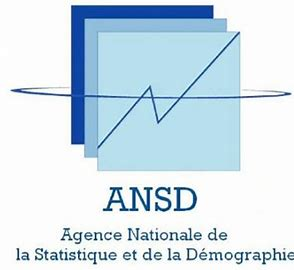
\includegraphics[width=\linewidth]{logo_ansd}
\end{minipage}
\hfill
\begin{minipage}{0.15\textwidth}

\includegraphics[width=\linewidth]{logo_ensae}
\end{minipage}

\vspace{2cm}

{\Huge\bfseries TP2 : Éducation et alphabétisation des membres des ménages \par}
\vspace{1.5cm}

{\Large\textbf{Rapport d'analyse}}\par
\vspace{1.5cm}

\textbf{Auteurs :}\par
\vspace{0.5cm}
Mouhamet SECK\\
\vspace{0.2cm}
Manampisoa Clarrat FINARITRINIAINA\\

\vfill

{\Large Projet statistique avec R ou python}\\
\vspace{1cm}
{\large ENSAE - ISE1-CL / ISE1 MATH - Mars 2026}

\vspace{1cm}

\end{center}
\end{titlepage}

{
\setcounter{tocdepth}{2}
\tableofcontents
}
\newpage

\section{Introduction}\label{introduction}

Ce rapport présente les analyses descriptives et les tests statistiques
réalisés dans le cadre du TP2, à partir des données de la Nigeria
General Household Survey (GHS) Panel -- vague 4 (2018--2019). L'objectif
est d'étudier les niveaux d'instruction et les taux d'alphabétisation
des membres des ménages nigérians, et de comparer les profils selon le
sexe, l'âge et la zone de résidence (urbain/rural).

\section{Méthodologie}\label{muxe9thodologie}

\subsection{Données et Variables
Clés}\label{donnuxe9es-et-variables-cluxe9s}

Les fichiers suivants ont été utilisés :

\begin{itemize}
\item
  \textbf{sect1\_harvestw4.dta} : 30 337 individus, variables
  démographiques (\texttt{s1q2} sexe, \texttt{s1q4} âge, \texttt{sector}
  milieu, \texttt{state} état).
\item
  \textbf{sect2\_harvestw4.dta} : 26 557 individus, module éducation
  (\texttt{s2aq5} alphabétisation, \texttt{s2aq6} a déjà été à l'école,
  \texttt{s2aq9} niveau d'éducation le plus élevé, \texttt{s2aq13a}
  scolarisation actuelle).
\item
  \textbf{secta\_harvestw4.dta} : 5 025 ménages, utilisé pour vérifier
  la couverture des identifiants.
\end{itemize}

Après vérification, aucun doublon n'est présent sur la clé
(\texttt{hhid}, \texttt{indiv}). Les ménages communs entre
\texttt{sect1} et \texttt{sect2} sont au nombre de 4 980, garantissant
une jointure fiable.

\subsection{Traitements Effectués}\label{traitements-effectuuxe9s}

\begin{Shaded}
\begin{Highlighting}[]
\CommentTok{\# Construction de la variable niveau d\textquotesingle{}éducation (5 catégories)}
\NormalTok{sect2\_educ }\OtherTok{\textless{}{-}}\NormalTok{ sect2\_w4 }\SpecialCharTok{\%\textgreater{}\%}
  \FunctionTok{mutate}\NormalTok{(}
    \AttributeTok{niveau\_educ =} \FunctionTok{case\_when}\NormalTok{(}
\NormalTok{      s2aq9 }\SpecialCharTok{\%in\%} \FunctionTok{c}\NormalTok{(}\DecValTok{0}\NormalTok{, }\DecValTok{1}\NormalTok{, }\DecValTok{2}\NormalTok{, }\DecValTok{3}\NormalTok{)       }\SpecialCharTok{\textasciitilde{}} \StringTok{"Aucun"}\NormalTok{,}
\NormalTok{      s2aq9 }\SpecialCharTok{\%in\%} \DecValTok{11}\SpecialCharTok{:}\DecValTok{16}               \SpecialCharTok{\textasciitilde{}} \StringTok{"Primaire"}\NormalTok{,}
\NormalTok{      s2aq9 }\SpecialCharTok{\%in\%} \DecValTok{21}\SpecialCharTok{:}\DecValTok{23}               \SpecialCharTok{\textasciitilde{}} \StringTok{"Junior Secondary"}\NormalTok{,}
\NormalTok{      s2aq9 }\SpecialCharTok{\%in\%} \FunctionTok{c}\NormalTok{(}\DecValTok{24}\SpecialCharTok{:}\DecValTok{28}\NormalTok{, }\DecValTok{321}\NormalTok{)       }\SpecialCharTok{\textasciitilde{}} \StringTok{"Senior Secondary"}\NormalTok{,}
\NormalTok{      s2aq9 }\SpecialCharTok{\%in\%} \FunctionTok{c}\NormalTok{(}\DecValTok{31}\NormalTok{, }\DecValTok{33}\NormalTok{, }\DecValTok{34}\NormalTok{, }\DecValTok{35}\NormalTok{,}
                   \DecValTok{41}\NormalTok{, }\DecValTok{43}\NormalTok{, }\DecValTok{322}\NormalTok{, }\DecValTok{411}\NormalTok{,}
                   \DecValTok{412}\NormalTok{, }\DecValTok{421}\SpecialCharTok{:}\DecValTok{424}\NormalTok{,}
                   \DecValTok{51}\NormalTok{, }\DecValTok{52}\NormalTok{, }\DecValTok{61}\NormalTok{)       }\SpecialCharTok{\textasciitilde{}} \StringTok{"Tertiaire"}\NormalTok{,}
      \ConstantTok{TRUE}                           \SpecialCharTok{\textasciitilde{}} \ConstantTok{NA\_character\_}
\NormalTok{    ),}
    \AttributeTok{niveau\_num =} \FunctionTok{case\_when}\NormalTok{(}
\NormalTok{      niveau\_educ }\SpecialCharTok{==} \StringTok{"Aucun"}             \SpecialCharTok{\textasciitilde{}} \DecValTok{0}\NormalTok{,}
\NormalTok{      niveau\_educ }\SpecialCharTok{==} \StringTok{"Primaire"}          \SpecialCharTok{\textasciitilde{}} \DecValTok{1}\NormalTok{,}
\NormalTok{      niveau\_educ }\SpecialCharTok{==} \StringTok{"Junior Secondary"}  \SpecialCharTok{\textasciitilde{}} \DecValTok{2}\NormalTok{,}
\NormalTok{      niveau\_educ }\SpecialCharTok{==} \StringTok{"Senior Secondary"}  \SpecialCharTok{\textasciitilde{}} \DecValTok{3}\NormalTok{,}
\NormalTok{      niveau\_educ }\SpecialCharTok{==} \StringTok{"Tertiaire"}         \SpecialCharTok{\textasciitilde{}} \DecValTok{4}\NormalTok{,}
      \ConstantTok{TRUE}                               \SpecialCharTok{\textasciitilde{}} \ConstantTok{NA\_real\_}
\NormalTok{    )}
\NormalTok{  )}

\CommentTok{\# Jointure avec les variables démographiques de sect1}
\NormalTok{educ\_demo }\OtherTok{\textless{}{-}}\NormalTok{ sect2\_educ }\SpecialCharTok{\%\textgreater{}\%}
  \FunctionTok{left\_join}\NormalTok{(}
\NormalTok{    sect1\_w4 }\SpecialCharTok{\%\textgreater{}\%} \FunctionTok{select}\NormalTok{(hhid, indiv, }\AttributeTok{sexe =}\NormalTok{ s1q2,}
                        \AttributeTok{age =}\NormalTok{ s1q4, }\AttributeTok{secteur =}\NormalTok{ sector, }\AttributeTok{etat =}\NormalTok{ state),}
    \AttributeTok{by =} \FunctionTok{c}\NormalTok{(}\StringTok{"hhid"}\NormalTok{, }\StringTok{"indiv"}\NormalTok{)}
\NormalTok{  )}

\CommentTok{\# Tests statistiques :}
\CommentTok{\#   {-} Chi{-}deux + V de Cramér : sexe × niveau d\textquotesingle{}éducation (adultes 18+)}
\CommentTok{\#   {-} Kruskal{-}Wallis : niveau d\textquotesingle{}éducation par groupe d\textquotesingle{}âge}
\CommentTok{\#   {-} Test post{-}hoc de Dunn (Bonferroni) : comparaisons multiples}
\CommentTok{\#   {-} Chi{-}deux : zone × scolarisation (enfants 6{-}17 ans)}
\end{Highlighting}
\end{Shaded}

Les traitements réalisés comprennent la construction d'une variable
ordonnée de niveau d'éducation en cinq catégories à partir des codes
détaillés de \texttt{s2aq9}, la jointure avec les variables
démographiques de \texttt{sect1}, et une série de tests statistiques :
chi-deux avec V de Cramér pour l'association sexe--niveau d'éducation,
test de Kruskal-Wallis suivi du test post-hoc de Dunn (correction de
Bonferroni) pour la comparaison du niveau d'éducation entre groupes
d'âge, et chi-deux pour l'association zone--scolarisation des enfants de
6 à 17 ans.

\section{Résultats}\label{ruxe9sultats}

\subsection{Qualité des Données et Valeurs
Manquantes}\label{qualituxe9-des-donnuxe9es-et-valeurs-manquantes}

L'examen des valeurs manquantes sur les variables clés révèle une
situation contrastée selon les fichiers. Dans \texttt{sect1\_w4}, les
variables démographiques (\texttt{s1q2}, \texttt{s1q4}, \texttt{sector},
\texttt{state}) sont quasi exhaustives avec moins de 0,5 \% de NA. Dans
\texttt{sect2\_w4}, les taux de manquants pour \texttt{s2aq5}
(alphabétisation) et \texttt{s2aq9} (niveau d'éducation) sont élevés
(environ 27 \%), ce qui est structurellement attendu : ces questions ne
s'adressent qu'aux personnes de 3 ans et plus, et les individus non
scolarisés n'ont pas de niveau d'éducation à déclarer. Les analyses
ultérieures ne portent que sur les individus ayant effectivement
répondu.

\subsection{Répartition du Niveau
d'Éducation}\label{ruxe9partition-du-niveau-duxe9ducation}

La distribution du niveau d'éducation le plus élevé, parmi les personnes
ayant répondu, est la suivante :

\begin{longtable}[]{@{}lrrl@{}}
\caption{Effectifs et proportions du niveau d'éducation}\tabularnewline
\toprule\noalign{}
niveau\_educ & n & prop & prop\_label \\
\midrule\noalign{}
\endfirsthead
\toprule\noalign{}
niveau\_educ & n & prop & prop\_label \\
\midrule\noalign{}
\endhead
\bottomrule\noalign{}
\endlastfoot
Primaire & 7068 & 0.367 & 36.7\% \\
Senior Secondary & 4617 & 0.240 & 24.0\% \\
Tertiaire & 3595 & 0.187 & 18.7\% \\
Junior Secondary & 2129 & 0.110 & 11.0\% \\
Aucun & 1862 & 0.097 & 9.7\% \\
\end{longtable}

\begin{center}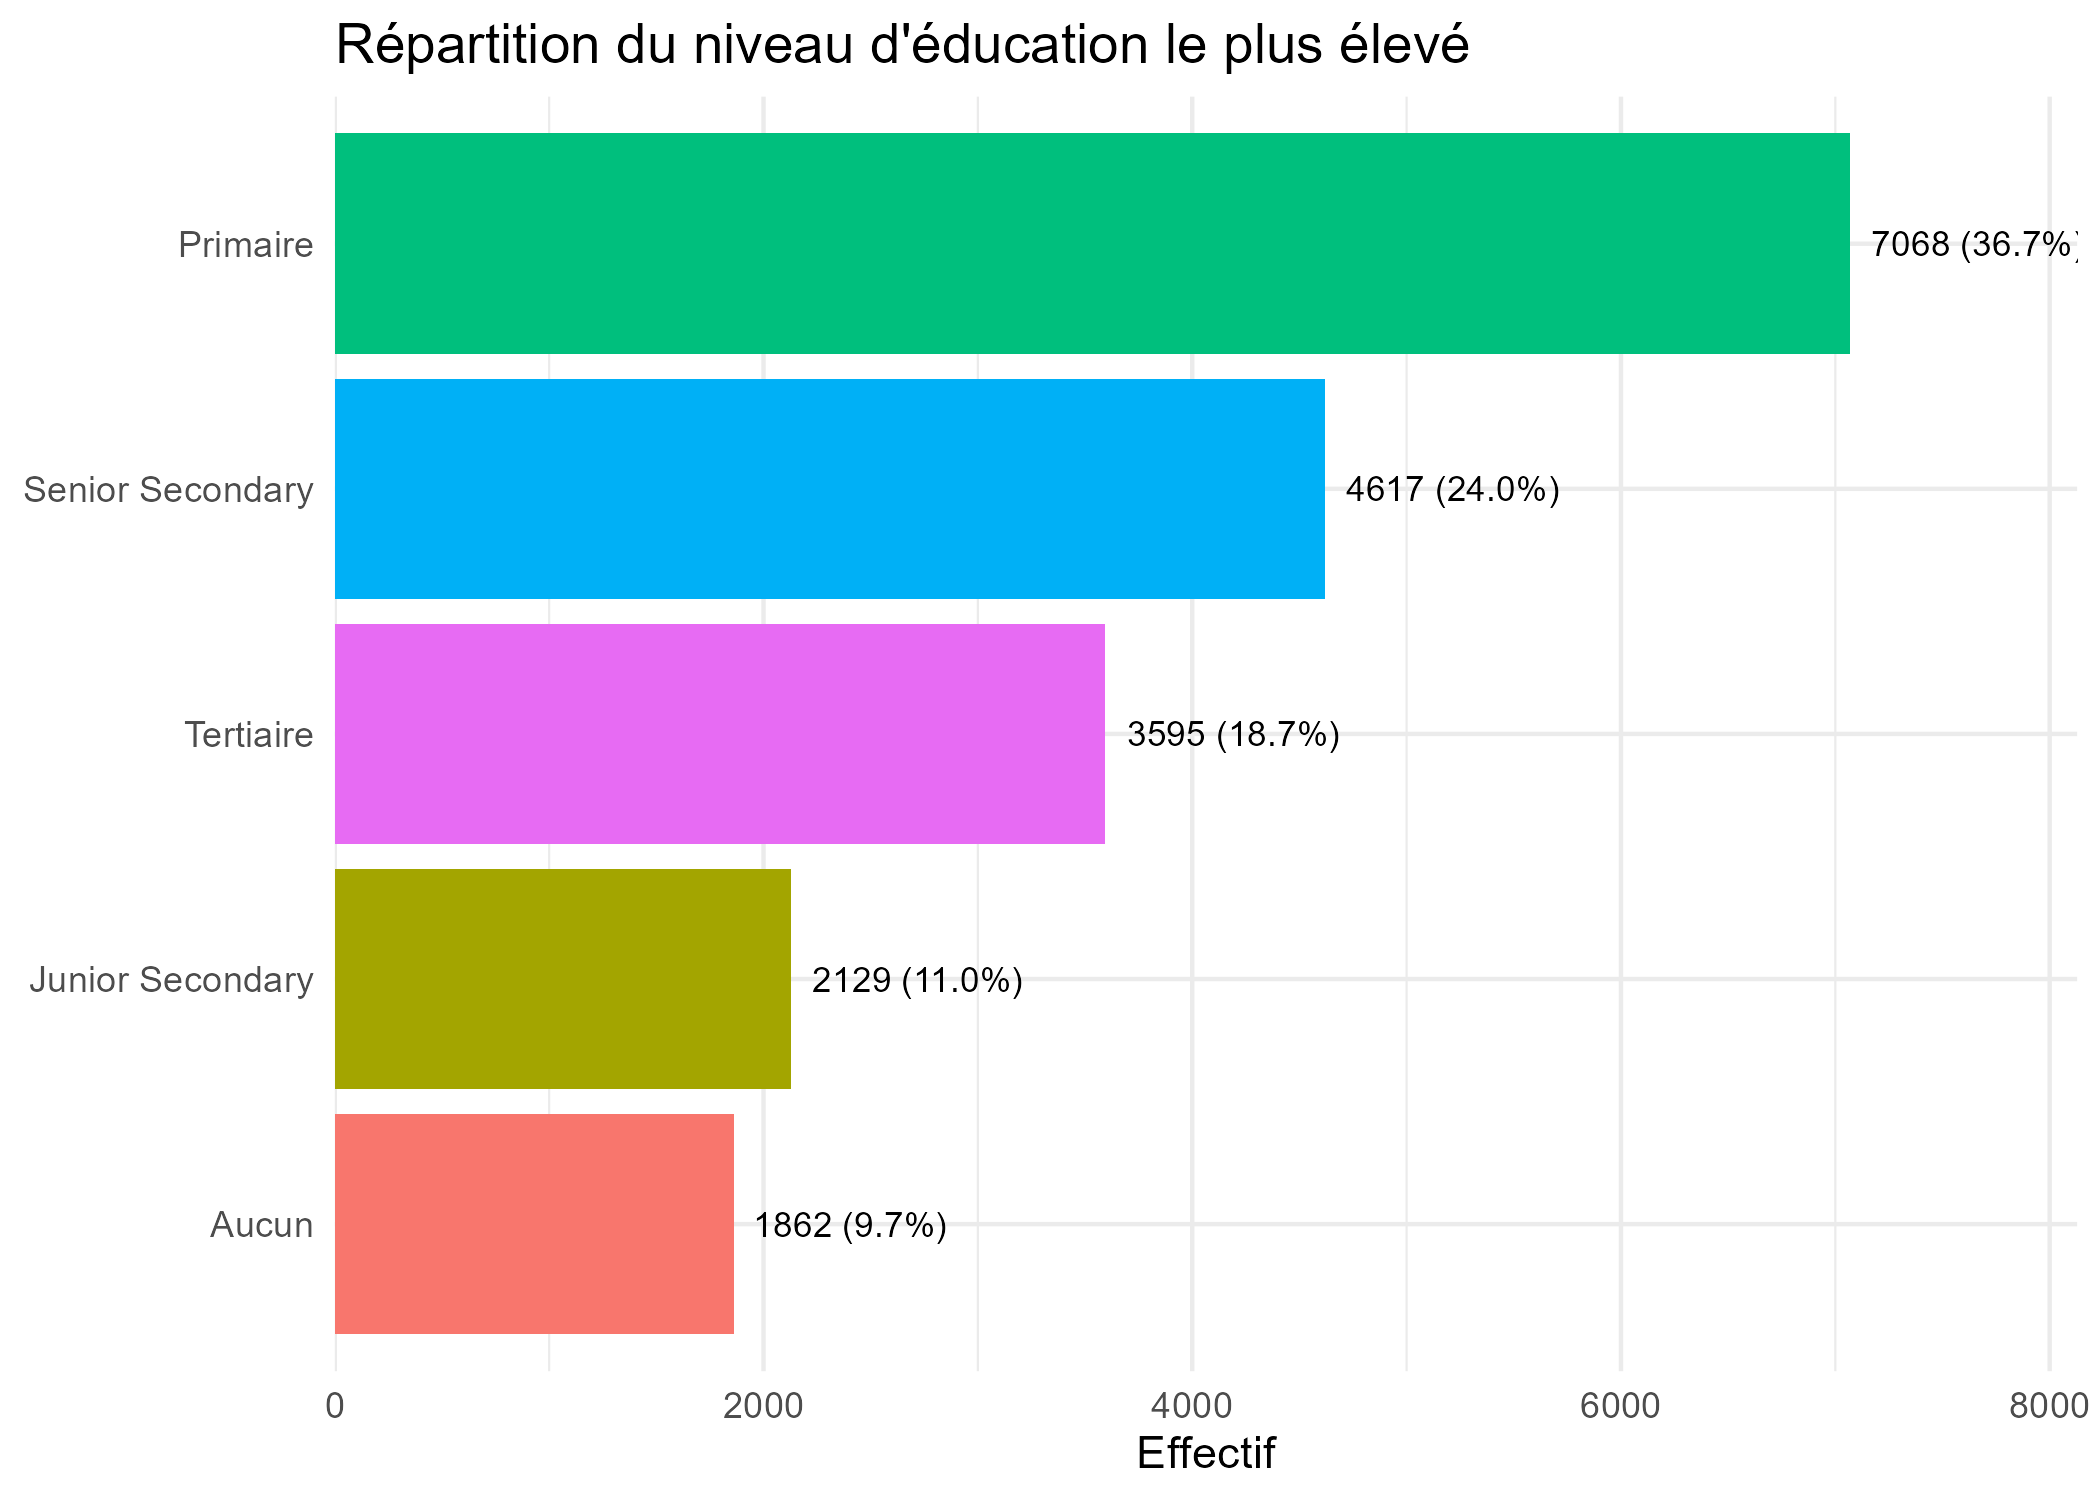
\includegraphics[width=1\linewidth]{../outputs/graphs/niveau_educ_barplot} \end{center}

Le niveau Primaire est le plus fréquent (36,7 \%), suivi du Senior
Secondary (24,0 \%) et du Tertiaire (18,7 \%). Les personnes sans aucune
instruction représentent 9,7 \% de l'échantillon. Ce profil reflète des
progrès importants dans l'accès à l'éducation de base, mais une
déperdition scolaire significative entre le primaire et les niveaux
supérieurs.

\subsection{Comparaison Hommes / Femmes (Adultes
18+)}\label{comparaison-hommes-femmes-adultes-18}

L'analyse porte sur les adultes de 18 ans et plus. Le tableau de
contingence croise le sexe et le niveau d'éducation.

\begin{longtable}[]{@{}lrrrrr@{}}
\caption{Tableau de contingence sexe × niveau d'éducation (adultes
18+)}\tabularnewline
\toprule\noalign{}
& Aucun & Primaire & Junior.Secondary & Senior.Secondary & Tertiaire \\
\midrule\noalign{}
\endfirsthead
\toprule\noalign{}
& Aucun & Primaire & Junior.Secondary & Senior.Secondary & Tertiaire \\
\midrule\noalign{}
\endhead
\bottomrule\noalign{}
\endlastfoot
Homme & 26 & 1198 & 359 & 2158 & 1690 \\
Femme & 47 & 1416 & 379 & 1687 & 1385 \\
\end{longtable}

\begin{center}
\includegraphics[width=1\linewidth]{../outputs/graphs/education_par_sexe} \end{center}

Le test du \(\chi^2\) est hautement significatif (p \textless{}
2,2e-16), indiquant une dépendance entre le sexe et le niveau
d'éducation. Le V de Cramér (0,092) correspond à une association faible
mais statistiquement robuste. Le graphique en barres 100 \% empilées
illustre la nature de cet écart : les hommes sont proportionnellement
plus nombreux dans les niveaux Senior Secondary et Tertiaire, tandis que
les femmes sont surreprésentées dans les niveaux Primaire et Aucun. Ces
inégalités de genre persistent malgré les progrès de la scolarisation
féminine au Nigeria, et reflètent des abandons scolaires plus précoces
chez les filles.

\subsection{Relation entre Âge et Niveau
d'Éducation}\label{relation-entre-uxe2ge-et-niveau-duxe9ducation}

Les adultes ont été regroupés en quatre tranches d'âge. Le boxplot
ci-dessous montre la distribution du niveau d'éducation (variable
numérique de 0 à 4) pour chaque groupe.

\begin{center}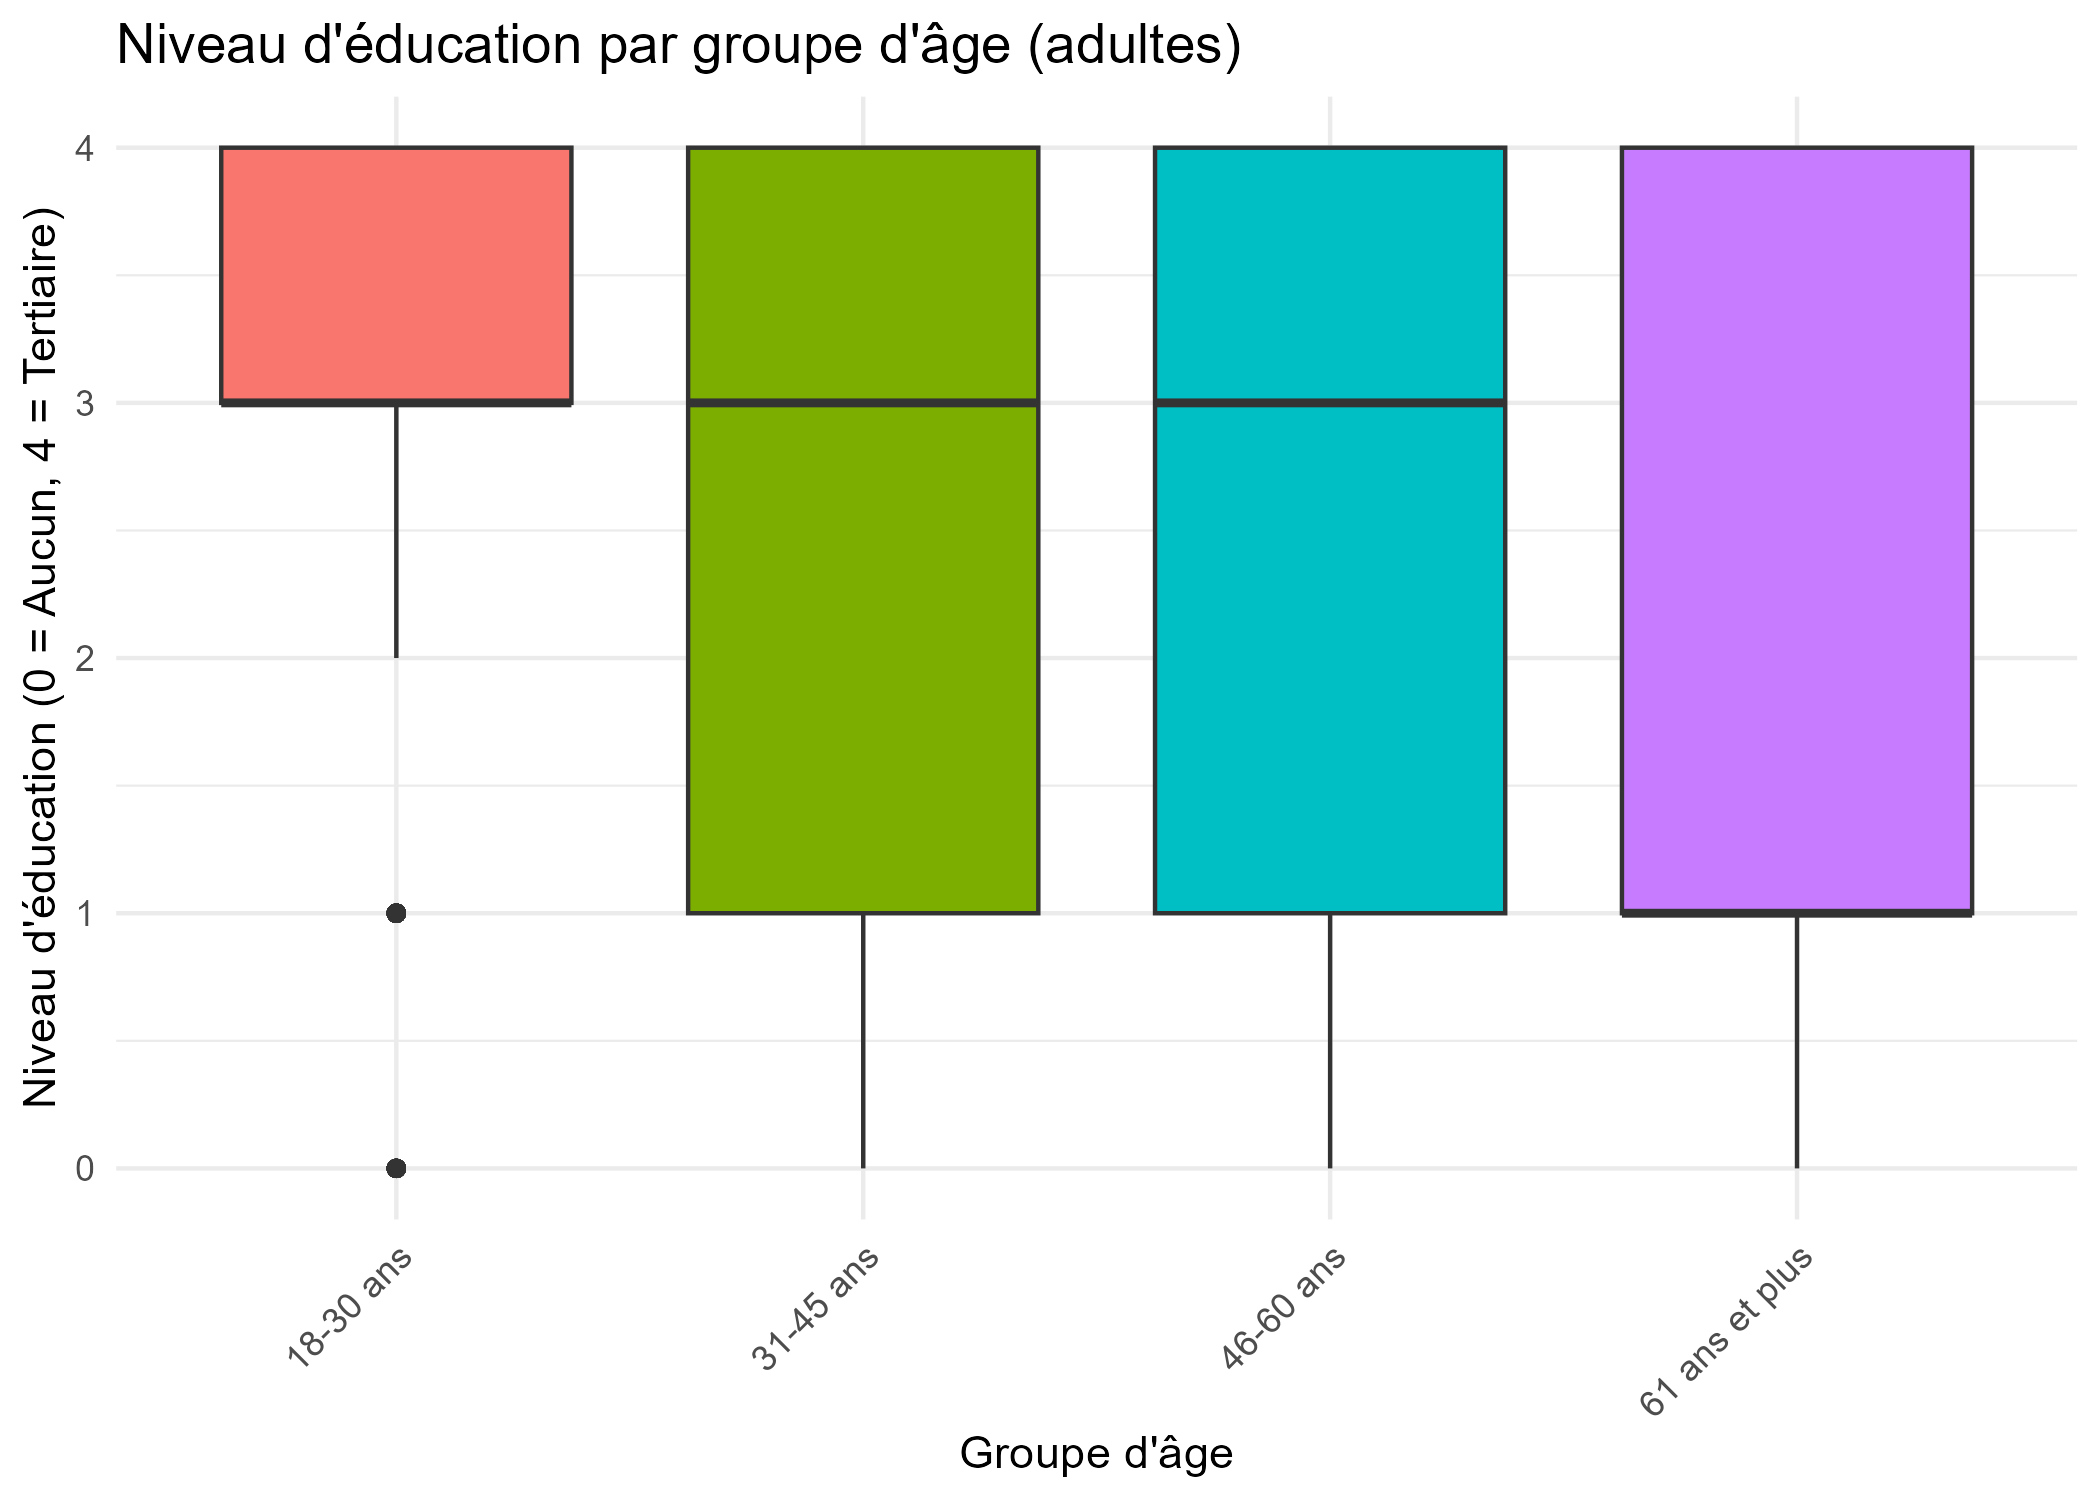
\includegraphics[width=1\linewidth]{../outputs/graphs/education_par_age_boxplot} \end{center}

\begin{longtable}[]{@{}lrrrr@{}}
\caption{Statistiques du niveau d'éducation par groupe
d'âge}\tabularnewline
\toprule\noalign{}
age\_group & n & mediane & Q1 & Q3 \\
\midrule\noalign{}
\endfirsthead
\toprule\noalign{}
age\_group & n & mediane & Q1 & Q3 \\
\midrule\noalign{}
\endhead
\bottomrule\noalign{}
\endlastfoot
18-30 ans & 4505 & 3 & 3 & 4 \\
31-45 ans & 3149 & 3 & 1 & 4 \\
46-60 ans & 1858 & 3 & 1 & 4 \\
61 ans et plus & 833 & 1 & 1 & 4 \\
\end{longtable}

Les jeunes adultes de 18--30 ans ont un niveau médian de 3 (Senior
Secondary), tandis que les 61 ans et plus affichent une médiane de 1
(Primaire). Cette progression générationnelle du niveau d'éducation
traduit les efforts d'expansion du système scolaire nigérian au cours
des dernières décennies. Le test de Kruskal-Wallis confirme une
différence très significative entre les groupes (p \textless{} 2,2e-16).

\begin{longtable}[]{@{}llrl@{}}
\caption{Test de Dunn -- comparaisons multiples par groupe d'âge
(correction Bonferroni)}\tabularnewline
\toprule\noalign{}
group1 & group2 & p.adj & p.adj.signif \\
\midrule\noalign{}
\endfirsthead
\toprule\noalign{}
group1 & group2 & p.adj & p.adj.signif \\
\midrule\noalign{}
\endhead
\bottomrule\noalign{}
\endlastfoot
18-30 ans & 31-45 ans & 0.0001403 & *** \\
18-30 ans & 46-60 ans & 0.0000000 & **** \\
18-30 ans & 61 ans et plus & 0.0000000 & **** \\
31-45 ans & 46-60 ans & 0.0161158 & * \\
31-45 ans & 61 ans et plus & 0.0000000 & **** \\
46-60 ans & 61 ans et plus & 0.0000265 & **** \\
\end{longtable}

Le test post-hoc de Dunn montre que tous les groupes d'âge diffèrent
significativement les uns des autres. Ces résultats confirment que le
gradient éducatif entre générations est graduel et statistiquement
robuste à chaque échelon.

\subsection{Taux de Scolarisation des 6--17 ans par
Zone}\label{taux-de-scolarisation-des-617-ans-par-zone}

La scolarisation est mesurée par la variable \texttt{s2aq13a}
(fréquentation scolaire actuelle) sur les enfants de 6 à 17 ans.

\begin{longtable}[]{@{}
  >{\raggedright\arraybackslash}p{(\linewidth - 14\tabcolsep) * \real{0.1077}}
  >{\raggedright\arraybackslash}p{(\linewidth - 14\tabcolsep) * \real{0.1538}}
  >{\raggedleft\arraybackslash}p{(\linewidth - 14\tabcolsep) * \real{0.0769}}
  >{\raggedleft\arraybackslash}p{(\linewidth - 14\tabcolsep) * \real{0.1692}}
  >{\raggedleft\arraybackslash}p{(\linewidth - 14\tabcolsep) * \real{0.0923}}
  >{\raggedleft\arraybackslash}p{(\linewidth - 14\tabcolsep) * \real{0.1077}}
  >{\raggedleft\arraybackslash}p{(\linewidth - 14\tabcolsep) * \real{0.1231}}
  >{\raggedright\arraybackslash}p{(\linewidth - 14\tabcolsep) * \real{0.1692}}@{}}
\caption{Effectifs et taux de scolarisation par zone}\tabularnewline
\toprule\noalign{}
\begin{minipage}[b]{\linewidth}\raggedright
zone
\end{minipage} & \begin{minipage}[b]{\linewidth}\raggedright
scolarise
\end{minipage} & \begin{minipage}[b]{\linewidth}\raggedleft
n
\end{minipage} & \begin{minipage}[b]{\linewidth}\raggedleft
total\_zone
\end{minipage} & \begin{minipage}[b]{\linewidth}\raggedleft
prop
\end{minipage} & \begin{minipage}[b]{\linewidth}\raggedleft
ic\_low
\end{minipage} & \begin{minipage}[b]{\linewidth}\raggedleft
ic\_high
\end{minipage} & \begin{minipage}[b]{\linewidth}\raggedright
prop\_label
\end{minipage} \\
\midrule\noalign{}
\endfirsthead
\toprule\noalign{}
\begin{minipage}[b]{\linewidth}\raggedright
zone
\end{minipage} & \begin{minipage}[b]{\linewidth}\raggedright
scolarise
\end{minipage} & \begin{minipage}[b]{\linewidth}\raggedleft
n
\end{minipage} & \begin{minipage}[b]{\linewidth}\raggedleft
total\_zone
\end{minipage} & \begin{minipage}[b]{\linewidth}\raggedleft
prop
\end{minipage} & \begin{minipage}[b]{\linewidth}\raggedleft
ic\_low
\end{minipage} & \begin{minipage}[b]{\linewidth}\raggedleft
ic\_high
\end{minipage} & \begin{minipage}[b]{\linewidth}\raggedright
prop\_label
\end{minipage} \\
\midrule\noalign{}
\endhead
\bottomrule\noalign{}
\endlastfoot
Rural & Non & 635 & 5515 & 0.115 & 0.107 & 0.124 & 11.5\% \\
Rural & Oui & 4880 & 5515 & 0.885 & 0.876 & 0.893 & 88.5\% \\
Urbain & Non & 179 & 2315 & 0.077 & 0.067 & 0.089 & 7.7\% \\
Urbain & Oui & 2136 & 2315 & 0.923 & 0.911 & 0.933 & 92.3\% \\
\end{longtable}

\begin{center}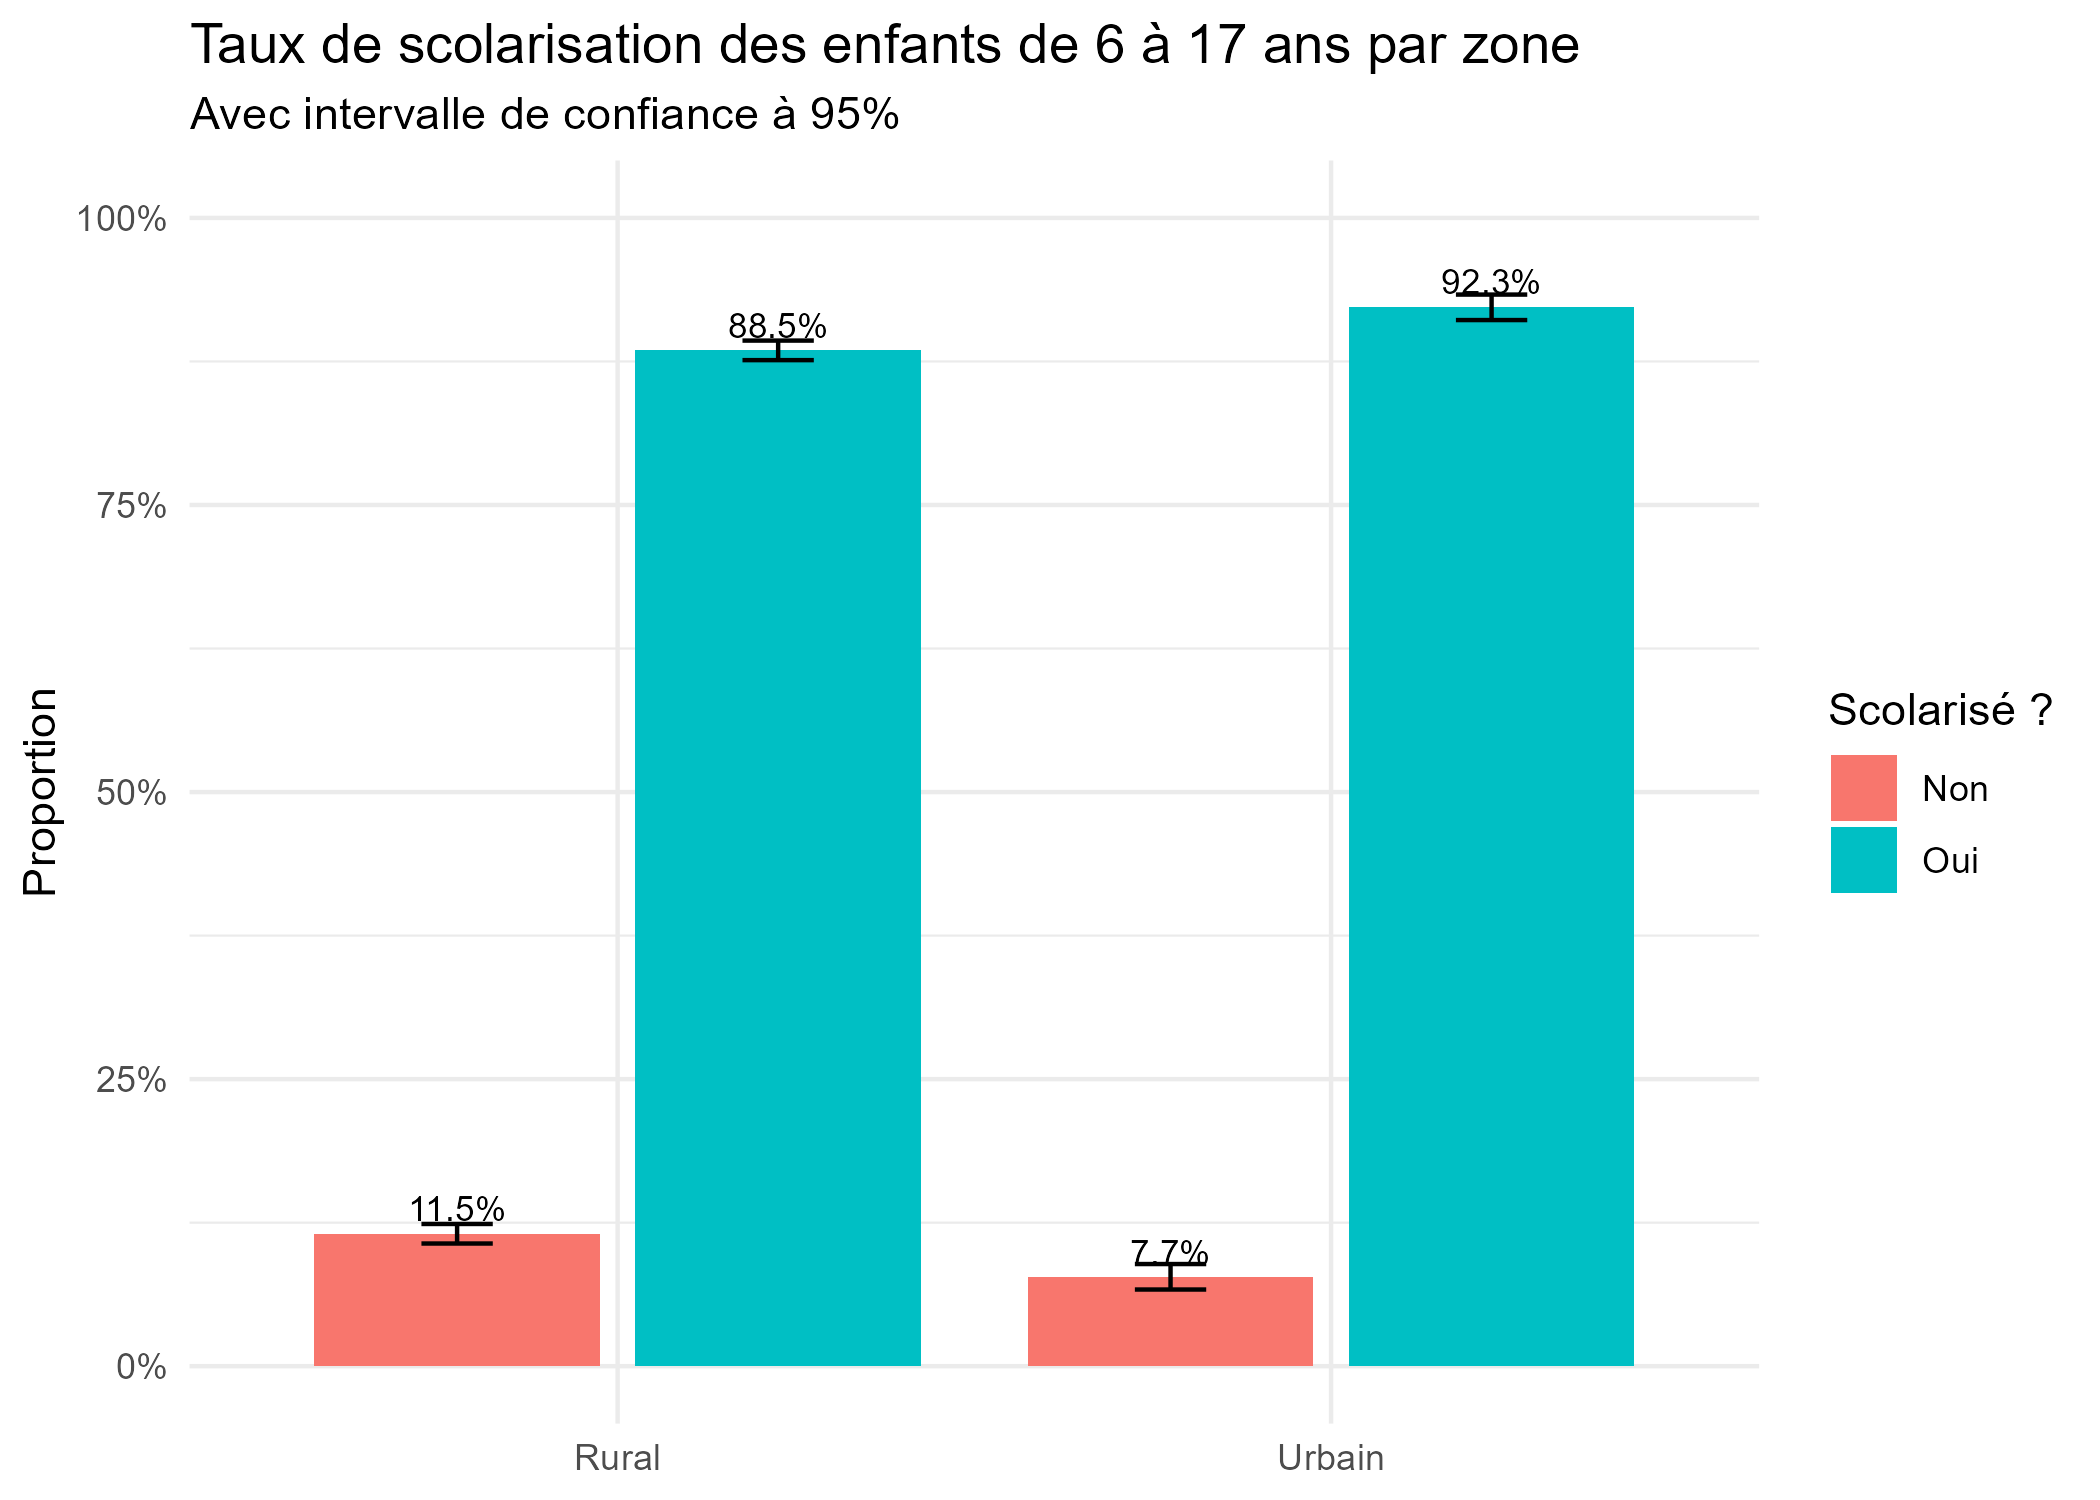
\includegraphics[width=1\linewidth]{../outputs/graphs/taux_scolarisation_par_zone_detail} \end{center}

Le taux de scolarisation est plus élevé en zone urbaine (92,3 \%) qu'en
zone rurale (88,5 \%), soit un écart de près de 4 points de pourcentage.
Les intervalles de confiance à 95 \% (méthode binomiale exacte) ne se
chevauchant pas, cette différence est statistiquement significative, ce
que confirme le test du \(\chi^2\) (p \textless{} 0,001). Si l'écart
reste modéré en valeur absolue, il suggère que les contraintes d'accès à
l'école -- distance, coûts directs et indirects, travail des enfants --
pèsent davantage en milieu rural.

\subsection{Carte du Taux d'Adultes sans Instruction par
État}\label{carte-du-taux-dadultes-sans-instruction-par-uxe9tat}

La proportion d'adultes (18 ans et plus) n'ayant aucun niveau
d'instruction a été calculée pour chaque État nigérian et reportée sur
une carte choroplèthe.

\begin{center}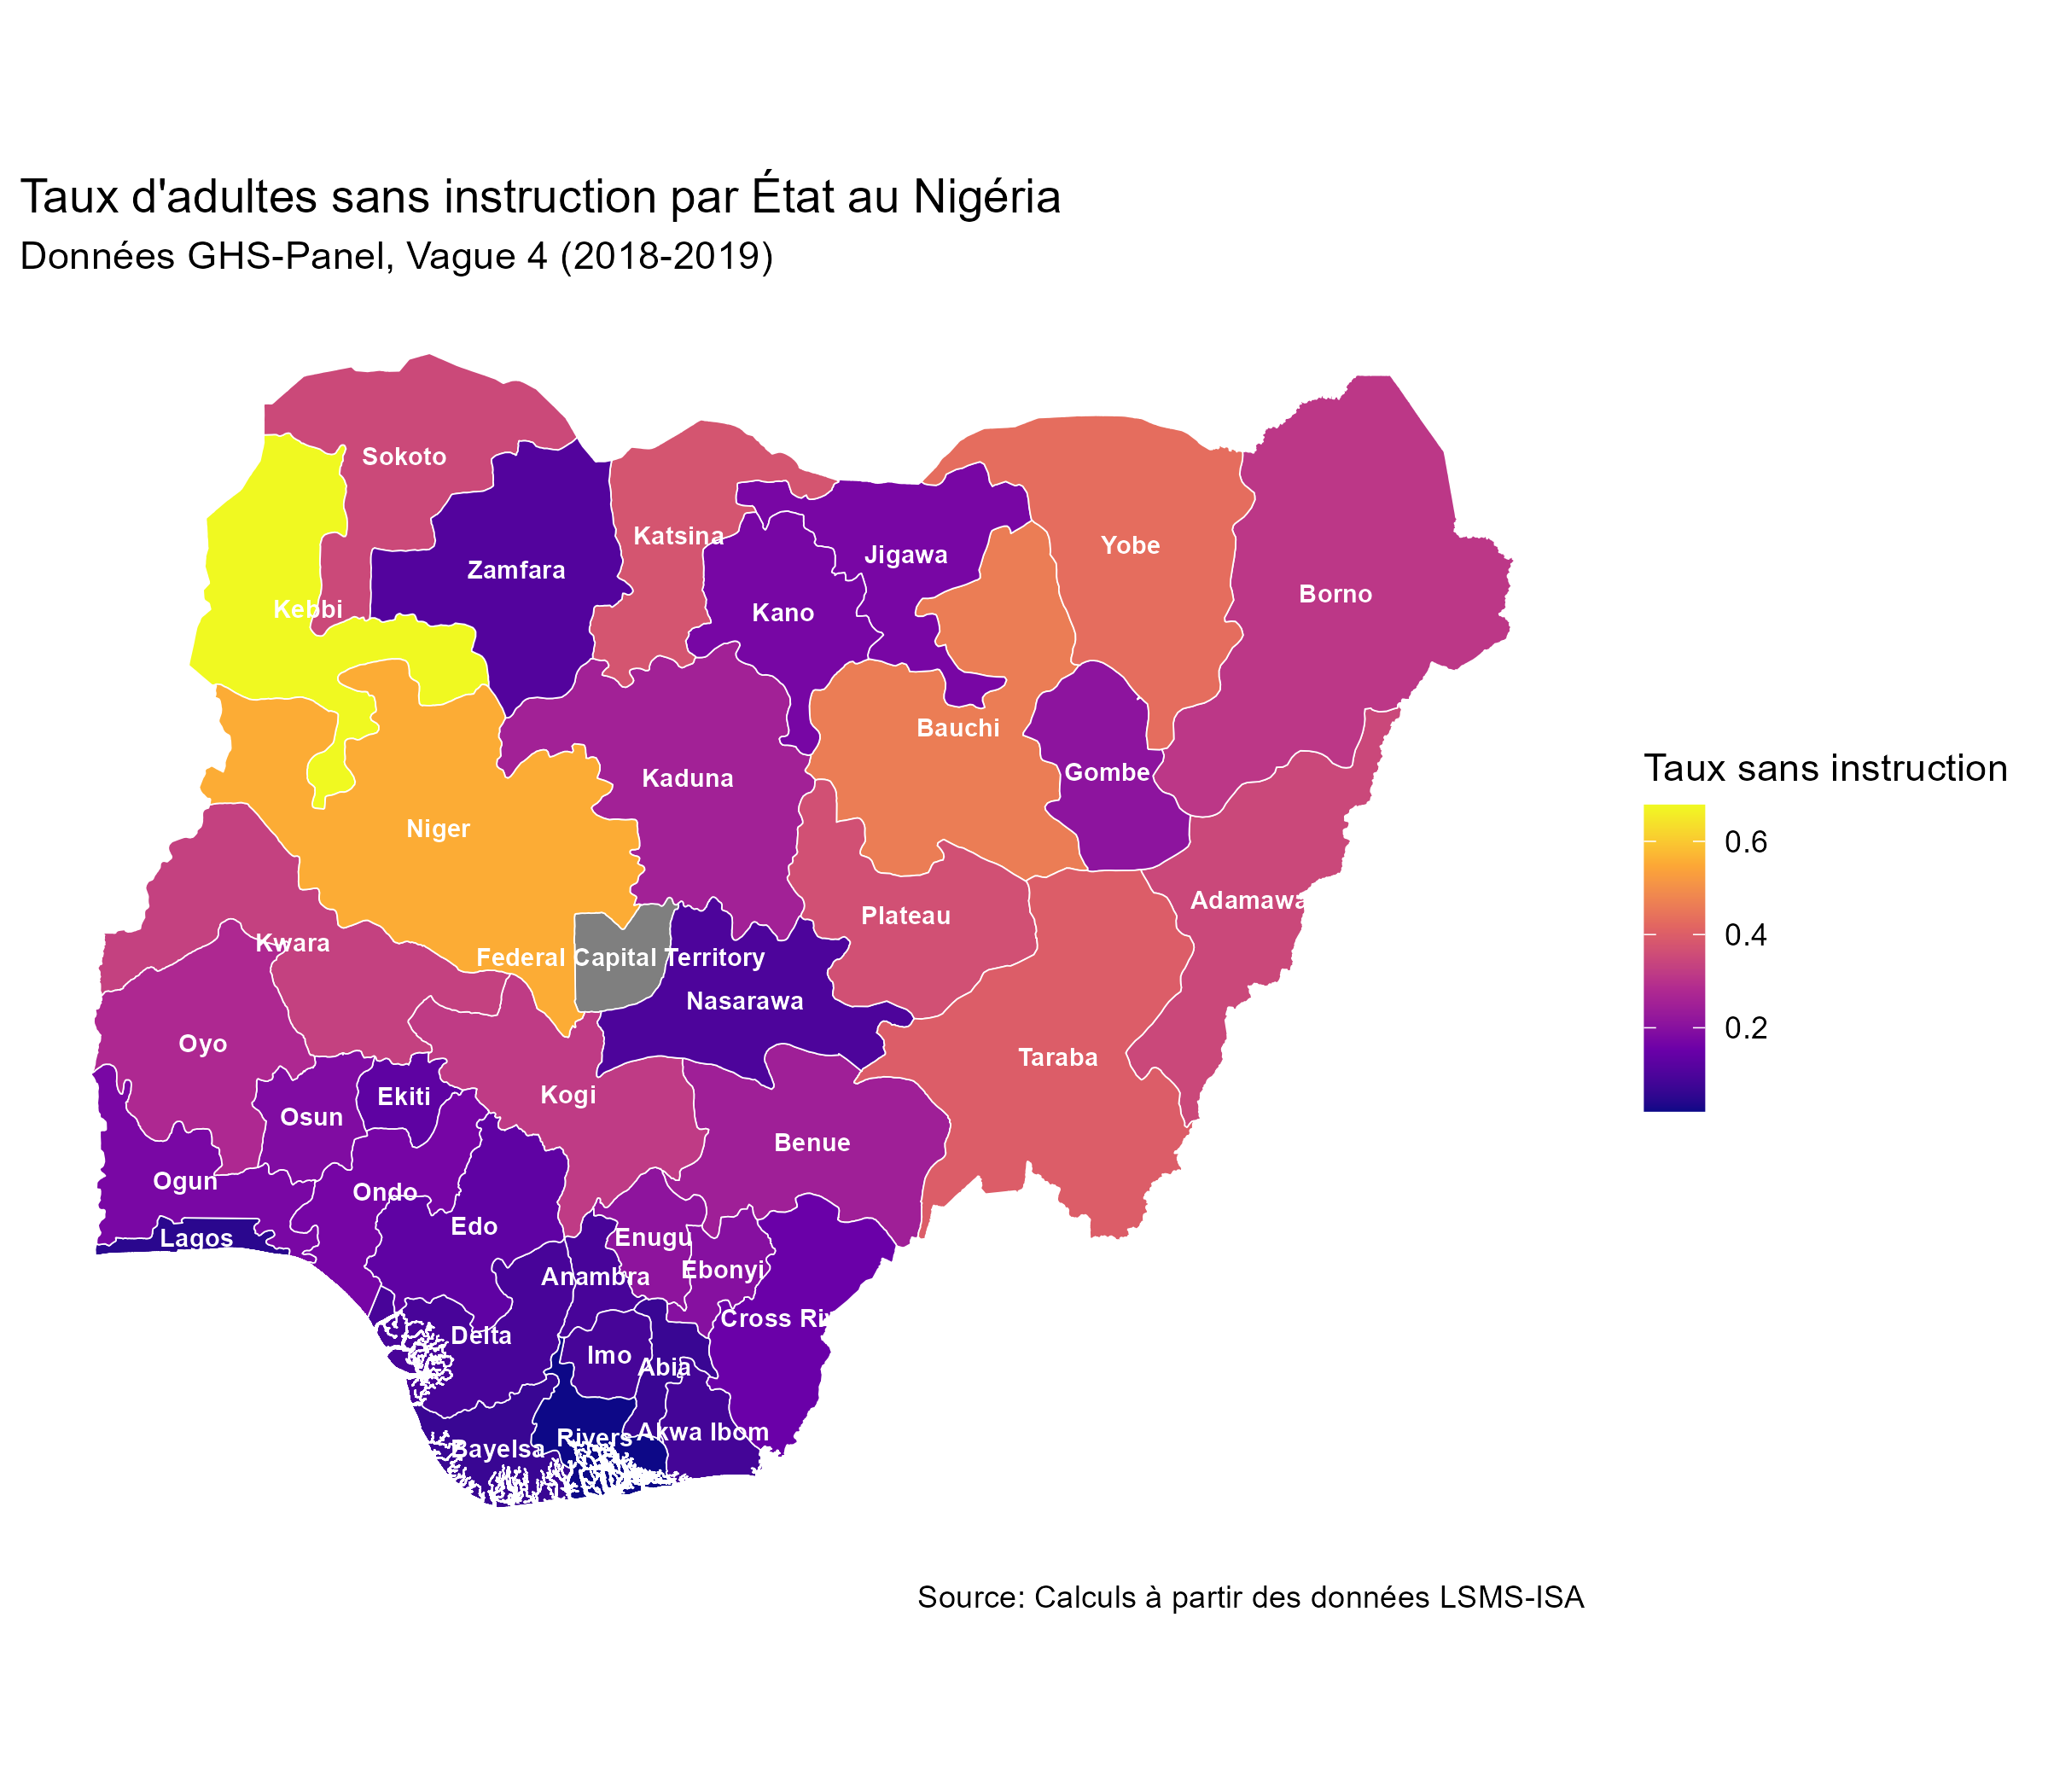
\includegraphics[width=1\linewidth]{../outputs/graphs/carte_taux_sans_instruction_avec_noms} \end{center}

Les États du Nord-Ouest notamment Sokoto et Kebbi affichent les taux les
plus élevés (proches de 60 \%), suivis des États du Nord-Est (Yobe,
Borno, Bauchi, entre 30 et 50 \%). À l'inverse, les États du Sud (Lagos,
Abia, Anambra, Rivers) présentent des taux inférieurs à 5 \%. Cette
fracture Nord-Sud reflète des inégalités historiques dans l'implantation
des infrastructures scolaires, renforcées par des facteurs culturels,
religieux et économiques. La zone FCT apparaît en gris en raison d'une
non-correspondance entre le nom dans les données et le shapefile, à
corriger si nécessaire.

\section{Discussion}\label{discussion}

Les analyses confirment des inégalités marquées en matière d'éducation
au Nigeria, selon trois axes principaux. Sur le plan du \textbf{genre},
les femmes adultes sont moins instruites que les hommes, avec une
surreprésentation dans les niveaux les plus bas et une
sous-représentation dans l'enseignement supérieur. Sur le plan
\textbf{générationnel}, les jeunes (18--30 ans) sont nettement plus
éduqués que les générations précédentes, témoignant des progrès de
l'accès à l'école au cours des dernières décennies, même si la
déperdition entre le primaire et les niveaux supérieurs reste
importante. Sur le plan \textbf{géographique}, de fortes disparités
régionales persistent, avec un retard structurel des États du Nord qui
concentrent l'essentiel des adultes sans instruction.

Ces trois axes d'inégalité se renforcent mutuellement : les États du
Nord sont aussi ceux où les inégalités de genre dans l'éducation sont
les plus prononcées, et où les taux de scolarisation des enfants --
notamment des filles -- sont les plus faibles. Toute politique éducative
efficace devra donc cibler simultanément ces dimensions géographiques,
de genre et générationnelles.

\textbf{Limites :}

\begin{itemize}
\item
  Les données sont déclaratives et peuvent souffrir de biais de mémoire,
  notamment pour la déclaration du niveau d'éducation des personnes
  âgées.
\item
  Les poids d'échantillonnage n'ont pas été utilisés ; les résultats
  sont donc représentatifs de l'échantillon mais pas nécessairement de
  la population nationale.
\item
  La variable d'alphabétisation (\texttt{s2aq5}) n'a pas été exploitée
  ici ; elle pourrait faire l'objet d'analyses complémentaires pour
  affiner le diagnostic éducatif.
\end{itemize}

\section{Conclusion}\label{conclusion}

Ce travail a permis de décrire la structure éducative de la population
nigériane à partir des données GHS-Panel vague 4. Il met en évidence des
progrès générationnels réels, mais aussi des inégalités persistantes
selon le sexe, le milieu de résidence et la région. La fracture Nord-Sud
constitue le défi structurel le plus important, tandis que les
inégalités de genre, bien que statistiquement significatives, semblent
s'atténuer dans les générations les plus jeunes. Ces résultats
constituent une base descriptive utile pour orienter les politiques
éducatives vers les populations et territoires les plus vulnérables.

\end{document}
